% Options for packages loaded elsewhere
\PassOptionsToPackage{unicode}{hyperref}
\PassOptionsToPackage{hyphens}{url}
\PassOptionsToPackage{dvipsnames,svgnames,x11names}{xcolor}
%
\documentclass[
  letterpaper,
  DIV=11,
  numbers=noendperiod]{scrartcl}

\usepackage{amsmath,amssymb}
\usepackage{iftex}
\ifPDFTeX
  \usepackage[T1]{fontenc}
  \usepackage[utf8]{inputenc}
  \usepackage{textcomp} % provide euro and other symbols
\else % if luatex or xetex
  \usepackage{unicode-math}
  \defaultfontfeatures{Scale=MatchLowercase}
  \defaultfontfeatures[\rmfamily]{Ligatures=TeX,Scale=1}
\fi
\usepackage{lmodern}
\ifPDFTeX\else  
    % xetex/luatex font selection
\fi
% Use upquote if available, for straight quotes in verbatim environments
\IfFileExists{upquote.sty}{\usepackage{upquote}}{}
\IfFileExists{microtype.sty}{% use microtype if available
  \usepackage[]{microtype}
  \UseMicrotypeSet[protrusion]{basicmath} % disable protrusion for tt fonts
}{}
\makeatletter
\@ifundefined{KOMAClassName}{% if non-KOMA class
  \IfFileExists{parskip.sty}{%
    \usepackage{parskip}
  }{% else
    \setlength{\parindent}{0pt}
    \setlength{\parskip}{6pt plus 2pt minus 1pt}}
}{% if KOMA class
  \KOMAoptions{parskip=half}}
\makeatother
\usepackage{xcolor}
\setlength{\emergencystretch}{3em} % prevent overfull lines
\setcounter{secnumdepth}{-\maxdimen} % remove section numbering
% Make \paragraph and \subparagraph free-standing
\ifx\paragraph\undefined\else
  \let\oldparagraph\paragraph
  \renewcommand{\paragraph}[1]{\oldparagraph{#1}\mbox{}}
\fi
\ifx\subparagraph\undefined\else
  \let\oldsubparagraph\subparagraph
  \renewcommand{\subparagraph}[1]{\oldsubparagraph{#1}\mbox{}}
\fi

\usepackage{color}
\usepackage{fancyvrb}
\newcommand{\VerbBar}{|}
\newcommand{\VERB}{\Verb[commandchars=\\\{\}]}
\DefineVerbatimEnvironment{Highlighting}{Verbatim}{commandchars=\\\{\}}
% Add ',fontsize=\small' for more characters per line
\usepackage{framed}
\definecolor{shadecolor}{RGB}{241,243,245}
\newenvironment{Shaded}{\begin{snugshade}}{\end{snugshade}}
\newcommand{\AlertTok}[1]{\textcolor[rgb]{0.68,0.00,0.00}{#1}}
\newcommand{\AnnotationTok}[1]{\textcolor[rgb]{0.37,0.37,0.37}{#1}}
\newcommand{\AttributeTok}[1]{\textcolor[rgb]{0.40,0.45,0.13}{#1}}
\newcommand{\BaseNTok}[1]{\textcolor[rgb]{0.68,0.00,0.00}{#1}}
\newcommand{\BuiltInTok}[1]{\textcolor[rgb]{0.00,0.23,0.31}{#1}}
\newcommand{\CharTok}[1]{\textcolor[rgb]{0.13,0.47,0.30}{#1}}
\newcommand{\CommentTok}[1]{\textcolor[rgb]{0.37,0.37,0.37}{#1}}
\newcommand{\CommentVarTok}[1]{\textcolor[rgb]{0.37,0.37,0.37}{\textit{#1}}}
\newcommand{\ConstantTok}[1]{\textcolor[rgb]{0.56,0.35,0.01}{#1}}
\newcommand{\ControlFlowTok}[1]{\textcolor[rgb]{0.00,0.23,0.31}{#1}}
\newcommand{\DataTypeTok}[1]{\textcolor[rgb]{0.68,0.00,0.00}{#1}}
\newcommand{\DecValTok}[1]{\textcolor[rgb]{0.68,0.00,0.00}{#1}}
\newcommand{\DocumentationTok}[1]{\textcolor[rgb]{0.37,0.37,0.37}{\textit{#1}}}
\newcommand{\ErrorTok}[1]{\textcolor[rgb]{0.68,0.00,0.00}{#1}}
\newcommand{\ExtensionTok}[1]{\textcolor[rgb]{0.00,0.23,0.31}{#1}}
\newcommand{\FloatTok}[1]{\textcolor[rgb]{0.68,0.00,0.00}{#1}}
\newcommand{\FunctionTok}[1]{\textcolor[rgb]{0.28,0.35,0.67}{#1}}
\newcommand{\ImportTok}[1]{\textcolor[rgb]{0.00,0.46,0.62}{#1}}
\newcommand{\InformationTok}[1]{\textcolor[rgb]{0.37,0.37,0.37}{#1}}
\newcommand{\KeywordTok}[1]{\textcolor[rgb]{0.00,0.23,0.31}{#1}}
\newcommand{\NormalTok}[1]{\textcolor[rgb]{0.00,0.23,0.31}{#1}}
\newcommand{\OperatorTok}[1]{\textcolor[rgb]{0.37,0.37,0.37}{#1}}
\newcommand{\OtherTok}[1]{\textcolor[rgb]{0.00,0.23,0.31}{#1}}
\newcommand{\PreprocessorTok}[1]{\textcolor[rgb]{0.68,0.00,0.00}{#1}}
\newcommand{\RegionMarkerTok}[1]{\textcolor[rgb]{0.00,0.23,0.31}{#1}}
\newcommand{\SpecialCharTok}[1]{\textcolor[rgb]{0.37,0.37,0.37}{#1}}
\newcommand{\SpecialStringTok}[1]{\textcolor[rgb]{0.13,0.47,0.30}{#1}}
\newcommand{\StringTok}[1]{\textcolor[rgb]{0.13,0.47,0.30}{#1}}
\newcommand{\VariableTok}[1]{\textcolor[rgb]{0.07,0.07,0.07}{#1}}
\newcommand{\VerbatimStringTok}[1]{\textcolor[rgb]{0.13,0.47,0.30}{#1}}
\newcommand{\WarningTok}[1]{\textcolor[rgb]{0.37,0.37,0.37}{\textit{#1}}}

\providecommand{\tightlist}{%
  \setlength{\itemsep}{0pt}\setlength{\parskip}{0pt}}\usepackage{longtable,booktabs,array}
\usepackage{calc} % for calculating minipage widths
% Correct order of tables after \paragraph or \subparagraph
\usepackage{etoolbox}
\makeatletter
\patchcmd\longtable{\par}{\if@noskipsec\mbox{}\fi\par}{}{}
\makeatother
% Allow footnotes in longtable head/foot
\IfFileExists{footnotehyper.sty}{\usepackage{footnotehyper}}{\usepackage{footnote}}
\makesavenoteenv{longtable}
\usepackage{graphicx}
\makeatletter
\def\maxwidth{\ifdim\Gin@nat@width>\linewidth\linewidth\else\Gin@nat@width\fi}
\def\maxheight{\ifdim\Gin@nat@height>\textheight\textheight\else\Gin@nat@height\fi}
\makeatother
% Scale images if necessary, so that they will not overflow the page
% margins by default, and it is still possible to overwrite the defaults
% using explicit options in \includegraphics[width, height, ...]{}
\setkeys{Gin}{width=\maxwidth,height=\maxheight,keepaspectratio}
% Set default figure placement to htbp
\makeatletter
\def\fps@figure{htbp}
\makeatother
\newlength{\cslhangindent}
\setlength{\cslhangindent}{1.5em}
\newlength{\csllabelwidth}
\setlength{\csllabelwidth}{3em}
\newlength{\cslentryspacingunit} % times entry-spacing
\setlength{\cslentryspacingunit}{\parskip}
\newenvironment{CSLReferences}[2] % #1 hanging-ident, #2 entry spacing
 {% don't indent paragraphs
  \setlength{\parindent}{0pt}
  % turn on hanging indent if param 1 is 1
  \ifodd #1
  \let\oldpar\par
  \def\par{\hangindent=\cslhangindent\oldpar}
  \fi
  % set entry spacing
  \setlength{\parskip}{#2\cslentryspacingunit}
 }%
 {}
\usepackage{calc}
\newcommand{\CSLBlock}[1]{#1\hfill\break}
\newcommand{\CSLLeftMargin}[1]{\parbox[t]{\csllabelwidth}{#1}}
\newcommand{\CSLRightInline}[1]{\parbox[t]{\linewidth - \csllabelwidth}{#1}\break}
\newcommand{\CSLIndent}[1]{\hspace{\cslhangindent}#1}

\usepackage{imakeidx} \makeindex \makeindex[name=authors, title=Authors, intoc=True] \makeindex[name=affiliations]
\KOMAoption{captions}{tableheading}
\makeatletter
\makeatother
\makeatletter
\makeatother
\makeatletter
\@ifpackageloaded{caption}{}{\usepackage{caption}}
\AtBeginDocument{%
\ifdefined\contentsname
  \renewcommand*\contentsname{Table of contents}
\else
  \newcommand\contentsname{Table of contents}
\fi
\ifdefined\listfigurename
  \renewcommand*\listfigurename{List of Figures}
\else
  \newcommand\listfigurename{List of Figures}
\fi
\ifdefined\listtablename
  \renewcommand*\listtablename{List of Tables}
\else
  \newcommand\listtablename{List of Tables}
\fi
\ifdefined\figurename
  \renewcommand*\figurename{Figure}
\else
  \newcommand\figurename{Figure}
\fi
\ifdefined\tablename
  \renewcommand*\tablename{Table}
\else
  \newcommand\tablename{Table}
\fi
}
\@ifpackageloaded{float}{}{\usepackage{float}}
\floatstyle{ruled}
\@ifundefined{c@chapter}{\newfloat{codelisting}{h}{lop}}{\newfloat{codelisting}{h}{lop}[chapter]}
\floatname{codelisting}{Listing}
\newcommand*\listoflistings{\listof{codelisting}{List of Listings}}
\makeatother
\makeatletter
\@ifpackageloaded{caption}{}{\usepackage{caption}}
\@ifpackageloaded{subcaption}{}{\usepackage{subcaption}}
\makeatother
\makeatletter
\@ifpackageloaded{tcolorbox}{}{\usepackage[skins,breakable]{tcolorbox}}
\makeatother
\makeatletter
\@ifundefined{shadecolor}{\definecolor{shadecolor}{rgb}{.97, .97, .97}}
\makeatother
\makeatletter
\makeatother
\makeatletter
\makeatother
\ifLuaTeX
  \usepackage{selnolig}  % disable illegal ligatures
\fi
\IfFileExists{bookmark.sty}{\usepackage{bookmark}}{\usepackage{hyperref}}
\IfFileExists{xurl.sty}{\usepackage{xurl}}{} % add URL line breaks if available
\urlstyle{same} % disable monospaced font for URLs
\hypersetup{
  pdftitle={Getting the hang of it},
  colorlinks=true,
  linkcolor={blue},
  filecolor={Maroon},
  citecolor={Blue},
  urlcolor={Blue},
  pdfcreator={LaTeX via pandoc}}

\title{Getting the hang of it}
\usepackage{etoolbox}
\makeatletter
\providecommand{\subtitle}[1]{% add subtitle to \maketitle
  \apptocmd{\@title}{\par {\large #1 \par}}{}{}
}
\makeatother
\subtitle{sprint 2}
\author{}
\date{19/05/2023}

\begin{document}
\maketitle
\ifdefined\Shaded\renewenvironment{Shaded}{\begin{tcolorbox}[sharp corners, boxrule=0pt, enhanced, borderline west={3pt}{0pt}{shadecolor}, interior hidden, breakable, frame hidden]}{\end{tcolorbox}}\fi

\renewcommand*\contentsname{Table of contents}
{
\hypersetup{linkcolor=}
\setcounter{tocdepth}{2}
\tableofcontents
}
\hypertarget{s02d01}{%
\subsection{{[}19-05-2023 / s02d01{]}}\label{s02d01}}

Objective for this second sprint:

\begin{itemize}
\tightlist
\item
  Description of finding labels for literature
\item
  Description of Design Science (prof Twente youtube die ook op seminar
  in Amsterdam was)
\item
  Description of DMAIC method, selectie projecten
\item
  Description of Python Measurement tool
\end{itemize}

Furhtermore I want to go back to sprint 1 to ``fix things''.
Specifically, I want to:

\begin{itemize}
\tightlist
\item
  take out some ideas and put these in a backlog (separate file).
\item
  improve the structure sucht that the sprint is more around the topic
  ``100 papers'' (even if I selected only 25)
\end{itemize}

Already the above seems like a lot for a 14 day sprint. Let's see where
we'll get \ldots{}

This will not appear in a HTML

\begin{figure}[H]

{\centering 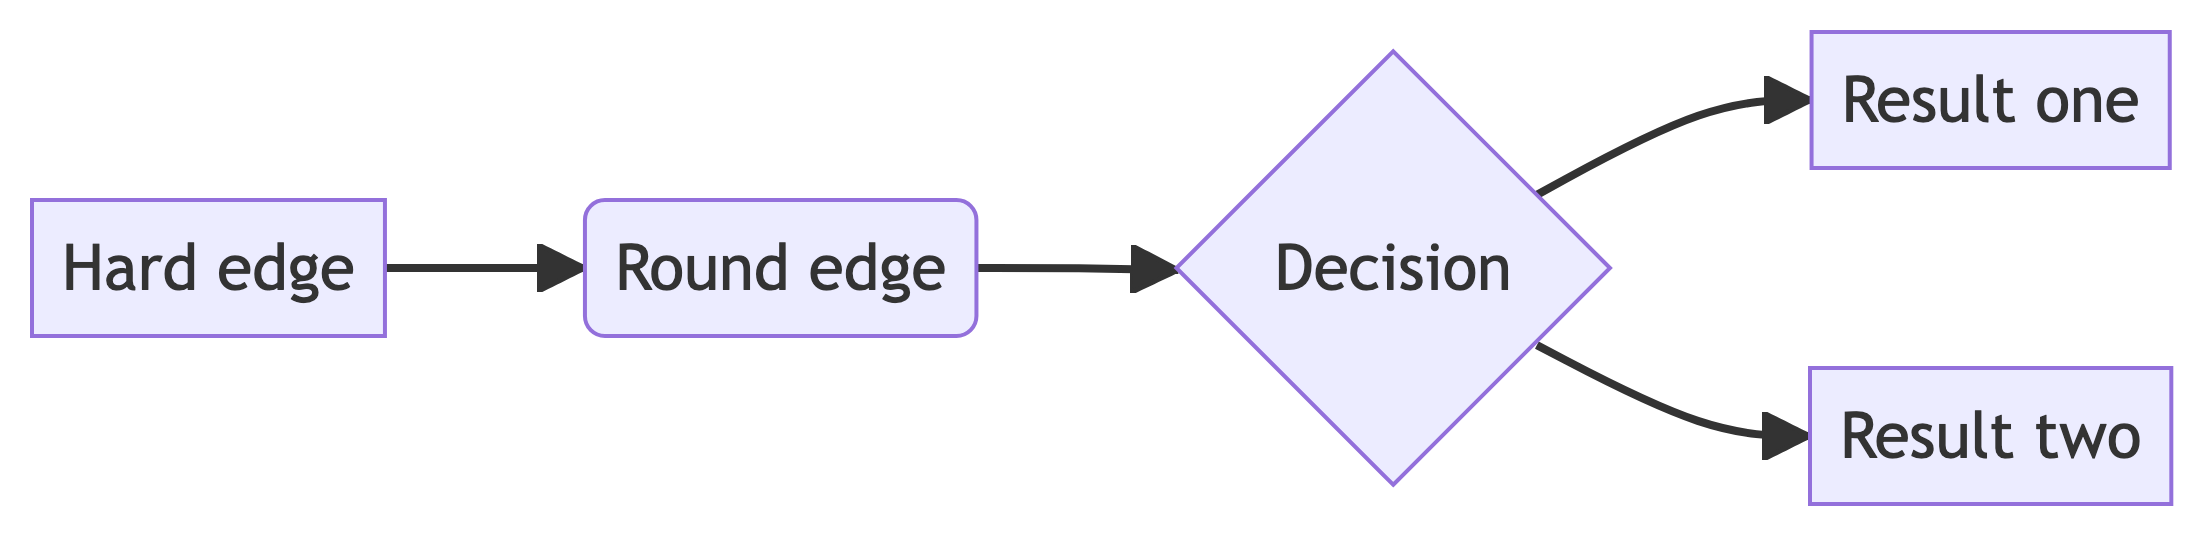
\includegraphics[width=5.74in,height=1.4in]{s3_methods_files/figure-latex/mermaid-figure-1.png}

}

\end{figure}

Use structurizer

\begin{longtable}[]{@{}
  >{\raggedright\arraybackslash}p{(\columnwidth - 16\tabcolsep) * \real{0.0345}}
  >{\raggedright\arraybackslash}p{(\columnwidth - 16\tabcolsep) * \real{0.1034}}
  >{\raggedright\arraybackslash}p{(\columnwidth - 16\tabcolsep) * \real{0.0230}}
  >{\raggedright\arraybackslash}p{(\columnwidth - 16\tabcolsep) * \real{0.0230}}
  >{\raggedright\arraybackslash}p{(\columnwidth - 16\tabcolsep) * \real{0.1609}}
  >{\raggedright\arraybackslash}p{(\columnwidth - 16\tabcolsep) * \real{0.1609}}
  >{\raggedright\arraybackslash}p{(\columnwidth - 16\tabcolsep) * \real{0.1724}}
  >{\raggedright\arraybackslash}p{(\columnwidth - 16\tabcolsep) * \real{0.2069}}
  >{\raggedright\arraybackslash}p{(\columnwidth - 16\tabcolsep) * \real{0.1149}}@{}}
\toprule\noalign{}
\begin{minipage}[b]{\linewidth}\raggedright
\#
\end{minipage} & \begin{minipage}[b]{\linewidth}\raggedright
Article
\end{minipage} & \begin{minipage}[b]{\linewidth}\raggedright
\end{minipage} & \begin{minipage}[b]{\linewidth}\raggedright
\end{minipage} & \begin{minipage}[b]{\linewidth}\raggedright
GSReferences
\end{minipage} & \begin{minipage}[b]{\linewidth}\raggedright
Published in
\end{minipage} & \begin{minipage}[b]{\linewidth}\raggedright
Journal Score
\end{minipage} & \begin{minipage}[b]{\linewidth}\raggedright
Principal Author
\end{minipage} & \begin{minipage}[b]{\linewidth}\raggedright
H-Factor
\end{minipage} \\
\midrule\noalign{}
\endhead
\bottomrule\noalign{}
\endlastfoot
\end{longtable}

\newpage{}

\hypertarget{s02d02-small-llm-to}{%
\subsection{{[}21-05-2023 / s02d02{]} Small LLM to
\ldots{}}\label{s02d02-small-llm-to}}

semantically query papers in the research database. For example see:

\begin{itemize}
\tightlist
\item
  \href{}{}
\item
  Dominik Weckmüller
  \href{https://geo.rocks/post/qdrant-transformers-js-semantic-search/}{Semantic
  Search with Qdrant, Hugging Face, SentenceTransformers and
  transformers.js}
\end{itemize}

\hypertarget{day02-authors-index}{%
\subsection{{[}20-05-2023 / day02{]} Authors
Index}\label{day02-authors-index}}

\hypertarget{day03-methodology}{%
\subsection{{[}21-05-2023 / day03{]}
Methodology}\label{day03-methodology}}

The paper recommended to my by email (per her email of ): \emph{Design
Science in Information Systems Research} (Hevner et al. 2004). Indeed,
in this write-up there are several papers where the Design Science
method is applied (Shafagatova and Van Looy 2021), \ldots{} (to be
continued).

Exemplars and criteria for applicable design science research (special
issue 2018 of the EJIS)

\begin{itemize}
\tightlist
\item
  also check: Christian Sonnenberg
\end{itemize}

(Cook and Sonnenberg 2014)

\hypertarget{day04-search-strategy}{%
\subsection{{[}22-05-2023 / day04{]} Search
strategy}\label{day04-search-strategy}}

Lets describe the search strategy

\begin{itemize}
\tightlist
\item
  one
\end{itemize}

\hypertarget{day07-lean-six-sigma}{%
\subsection{{[}25-05-2024 / day07{]} Lean Six
Sigma}\label{day07-lean-six-sigma}}

DMAIC

Voorbeeld

\begin{itemize}
\tightlist
\item
  to be excluded in pdf
\item
  to be included in pdf
\end{itemize}

\subsection{R}

\begin{Shaded}
\begin{Highlighting}[]
\NormalTok{fizz\_buzz }\OtherTok{\textless{}{-}} \ControlFlowTok{function}\NormalTok{(}\AttributeTok{fbnums =} \DecValTok{1}\SpecialCharTok{:}\DecValTok{50}\NormalTok{) \{}
\NormalTok{  output }\OtherTok{\textless{}{-}}\NormalTok{ dplyr}\SpecialCharTok{::}\FunctionTok{case\_when}\NormalTok{(}
\NormalTok{    fbnums }\SpecialCharTok{\%\%} \DecValTok{15} \SpecialCharTok{==} \DecValTok{0} \SpecialCharTok{\textasciitilde{}} \StringTok{"FizzBuzz"}\NormalTok{,}
\NormalTok{    fbnums }\SpecialCharTok{\%\%} \DecValTok{3} \SpecialCharTok{==} \DecValTok{0} \SpecialCharTok{\textasciitilde{}} \StringTok{"Fizz"}\NormalTok{,}
\NormalTok{    fbnums }\SpecialCharTok{\%\%} \DecValTok{5} \SpecialCharTok{==} \DecValTok{0} \SpecialCharTok{\textasciitilde{}} \StringTok{"Buzz"}\NormalTok{,}
    \ConstantTok{TRUE} \SpecialCharTok{\textasciitilde{}} \FunctionTok{as.character}\NormalTok{(fbnums)}
\NormalTok{  )}
  \FunctionTok{print}\NormalTok{(output)}
\NormalTok{\}}
\end{Highlighting}
\end{Shaded}

\subsection{Python}

\begin{Shaded}
\begin{Highlighting}[]
\KeywordTok{def}\NormalTok{ fizz\_buzz(num):}
  \ControlFlowTok{if}\NormalTok{ num }\OperatorTok{\%} \DecValTok{15} \OperatorTok{==} \DecValTok{0}\NormalTok{:}
    \BuiltInTok{print}\NormalTok{(}\StringTok{"FizzBuzz"}\NormalTok{)}
  \ControlFlowTok{elif}\NormalTok{ num }\OperatorTok{\%} \DecValTok{5} \OperatorTok{==} \DecValTok{0}\NormalTok{:}
    \BuiltInTok{print}\NormalTok{(}\StringTok{"Buzz"}\NormalTok{)}
  \ControlFlowTok{elif}\NormalTok{ num }\OperatorTok{\%} \DecValTok{3} \OperatorTok{==} \DecValTok{0}\NormalTok{:}
    \BuiltInTok{print}\NormalTok{(}\StringTok{"Fizz"}\NormalTok{)}
  \ControlFlowTok{else}\NormalTok{:}
    \BuiltInTok{print}\NormalTok{(num)}
\end{Highlighting}
\end{Shaded}

\hypertarget{day9-toepassing-voor-geopandas}{%
\subsection{{[}27-05-2024 / day9{]} Toepassing voor
GeoPandas?}\label{day9-toepassing-voor-geopandas}}

Bestand met locaties van universiteiten?

\hypertarget{day10-examples-of-design-science}{%
\subsection{{[}28-05-2023 / day10{]} Examples of Design
Science}\label{day10-examples-of-design-science}}

Design Science in Information System Research (Hevner et al. 2004)
written by Hevner et
al.~\index[authors]{Hevner, Alan R. \social[googlescholar]{john.doe}}

Getting Personal: A Deep Learning Artifact for Text-based Measurement of
Personality

\hypertarget{day11-process-modelling}{%
\subsection{{[}29-05-2023 / day11{]} Process
Modelling}\label{day11-process-modelling}}

(Mendling, Reijers, and van der Aalst 2010) written by

(Li 2010)

(Vicente-Saez and Martinez-Fuentes 2018)

\hypertarget{refs}{}
\begin{CSLReferences}{1}{0}
\leavevmode\vadjust pre{\hypertarget{ref-cookTechnologyOnlineEducation2014}{}}%
Cook, Catherine W, and Christian Sonnenberg. 2014. {``Technology and
Online Education: {Models} for Change.''} \emph{Contemporary Issues in
Education Research (CIER)} 7 (3): 171--88.

\leavevmode\vadjust pre{\hypertarget{ref-hevnerDesignScienceInformation2004}{}}%
Hevner, Alan R., Salvatore T. March, Jinsoo Park, and Sudha Ram. 2004.
{``Design Science in Information Systems Research.''} Journal
\{\{Article\}\}. \emph{MIS Quarterly}, 75--105.

\leavevmode\vadjust pre{\hypertarget{ref-liTextualAnalysisCorporate2010}{}}%
Li, Feng. 2010. {``Textual {Analysis} of {Corporate Disclosures}: {A
Survey} of the {Literature}.''} \emph{Journal of Accounting Literature}
29: 143--65.

\leavevmode\vadjust pre{\hypertarget{ref-mendlingSevenProcessModeling2010}{}}%
Mendling, J., H. A. Reijers, and W. M. P. van der Aalst. 2010. {``Seven
Process Modeling Guidelines ({7PMG}).''} \emph{Information and Software
Technology} 52 (2): 127--36.
\url{https://doi.org/10.1016/j.infsof.2009.08.004}.

\leavevmode\vadjust pre{\hypertarget{ref-shafagatovaDevelopingToolProcess2021}{}}%
Shafagatova, Aygun, and Amy Van Looy. 2021. {``Developing a Tool for
Process-Oriented Appraisals and Rewards: {Design} Science Research.''}
\emph{Journal of Software: Evolution and Process} 33 (3): e2321.

\leavevmode\vadjust pre{\hypertarget{ref-VICENTESAEZ2018428}{}}%
Vicente-Saez, Ruben, and Clara Martinez-Fuentes. 2018. {``Open {Science}
Now: {A} Systematic Literature Review for an Integrated Definition.''}
\emph{Journal of Business Research} 88: 428--36.
\url{https://doi.org/10.1016/j.jbusres.2017.12.043}.

\end{CSLReferences}



\printindex \printindex[authors]

\end{document}
